\documentclass[aspectratio=169]{beamer}

\setbeameroption{show notes on second screen}

\usepackage[utf8]{inputenc}
\usetheme{Madrid}
\usecolortheme{beaver}

\usepackage{graphicx}
\graphicspath{ {./Resources/} }

% Title here
\title{SNUB, The SNHU Student Database}
\author{Tim, Ben, Joe, Max}
\institute{SNHU CS-114}

\begin{document}

\frame{\titlepage} % Draw the title page

\begin{frame}
    \frametitle{Introduction}

    \begin{center}
     
\includegraphics[width=11cm]{harold}
    \end{center}

    \note{
        \huge{Ben}\normalsize

        We made a database that stores information online and sends that to your computer
    }
\end{frame}

\begin{frame}
    \frametitle{Features}

    
    \begin{block}{\centering C\# Was Used to Develop the Following Testing Environment:}
    \end{block}
    % Some columns
    \begin{columns}
        \begin{column}{0.3\textwidth}
            \begin{block}{Users are Directed to:}
            \begin{itemize}
                \item Connect to the server
                \item Select a class from a drop-down menu
                \item Select a note from the list box.
            \end{itemize}
            \end{block}
        \end{column}
        \begin{column}{0.48\textwidth}
            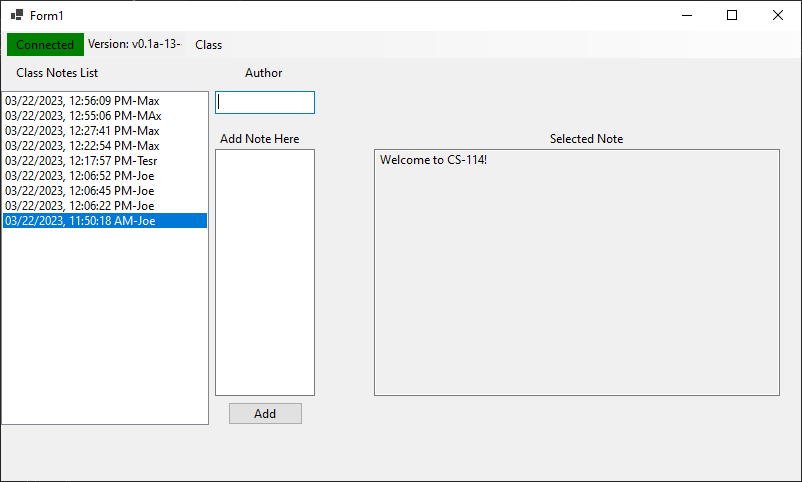
\includegraphics[width=8cm]{Sample_of_Features}
        \end{column}
    \end{columns}

    \note{
        \huge{Max}\normalsize

        Put note here
    }
\end{frame}

\begin{frame}
    \frametitle{Features (Server)}

    \begin{block}{\centering Connect to Server Feature}
        \centering 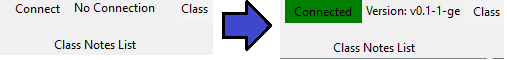
\includegraphics [width=9cm] {connect_to_connected.png}
    \end{block}
    \centering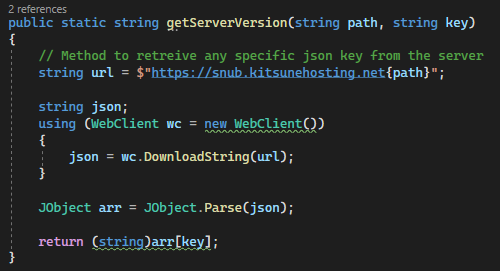
\includegraphics [width=9cm] {getServerVersion.PNG}

    \note{
        \huge{Joe}\normalsize

        One of the main features of our app, is its ability to connect to a centralized
        server and display information from other users.

        Users can connect to the server, to get the latest information about any class.
    }
\end{frame}

\begin{frame}
    \frametitle{Features (Selecting Class)}

    \begin{block}{\centering Select a Class Feature}
        \centering Users are Directed to select a class from the drop-down menu. This populates the class notes list box with the date and author of each note corresponding to the selected class.
    \end{block}

    \centering 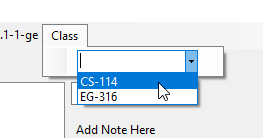
\includegraphics [width=10cm] {select}

    \note{
        \huge{Max}\normalsize

        Put note here
    }
\end{frame}

\begin{frame}
    \frametitle{Features (Populate notes)}

    \begin{block}{\centering Populate Selected Note Feature}
        \centering Users may select an item from the list box to populate the selected note text box.
    \end{block}

    \centering 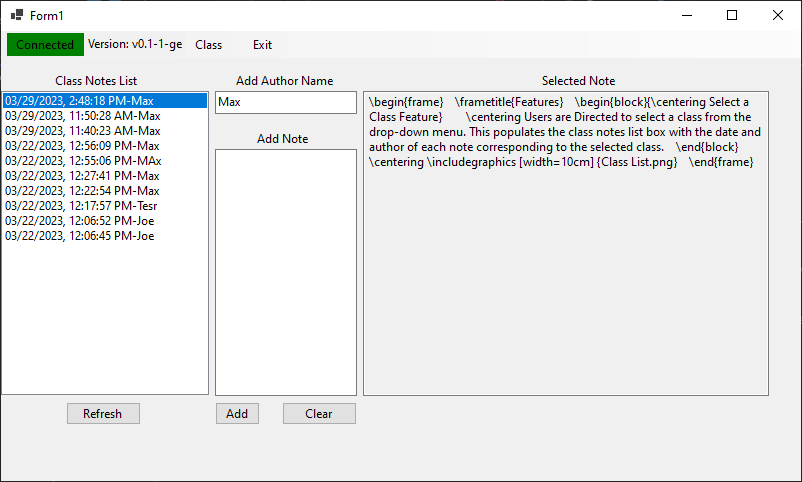
\includegraphics[height=5cm]{Select Class Note.png}
    
    \note{
        \huge{Ben}\normalsize

        The previously added notes appear and when clicked, fills the note
        text textbox.
    }
\end{frame}

\begin{frame}
    \frametitle{Features (Add note)}

    \begin{block}{\centering Add Note Feature}
        \centering Users may add a note to the database by adding text to both the author and add note text boxes. If the user attempts to add a note containing an empty string they are prompted to try again.
    \end{block}

    \centering 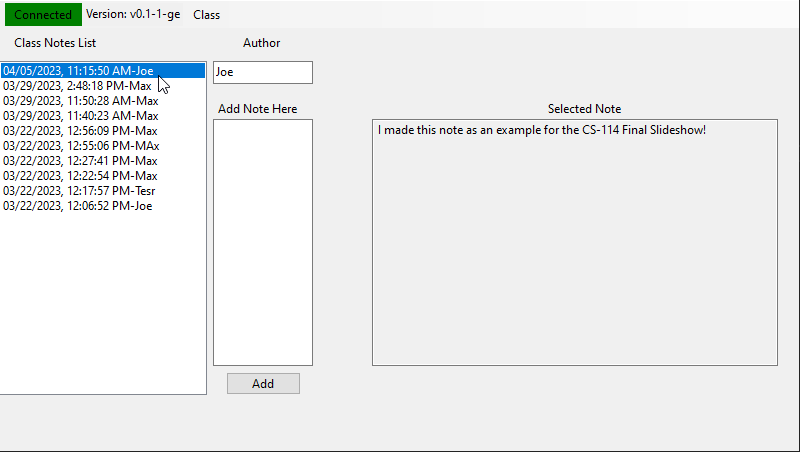
\includegraphics[height=5cm]{created.png}

    \note{
        \huge{Max}\normalsize

        Put note here
    }
\end{frame}

\begin{frame}
    \frametitle{Network and Database}

    % Some columns
    \begin{columns}
        \begin{column}{0.48\textwidth}
            \begin{block}{Data storage and Acquisition}
                All data is stored in a server, allowing for multiple clients. Data acquisition occurs as needed during use through a series of methods developed in c\#.
            \end{block}
        \end{column}
        \begin{column}{0.48\textwidth}
            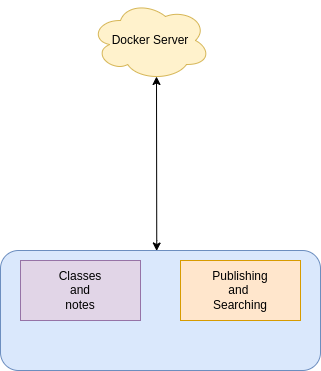
\includegraphics[width=5cm]{Simple Diagram.png}
        \end{column}
    \end{columns}

    \note{
        \huge{Joe}\normalsize

        All the data for SNUB is stored on the server. Allowing everyone to access it,
        the server is a docker container and a sql container running side by side on
        the internet. We use C\# to communicate back to the server, and retreive or set
        data.
    }
\end{frame}

\begin{frame}
    \frametitle{Github}

    % Some columns
    \begin{columns}
        \begin{column}{0.28\textwidth}
            \begin{block}{Github}
                We use github to build, check and publish both our docker images and the installer for our client.
            \end{block}
        \end{column}
        \begin{column}{0.58\textwidth}
            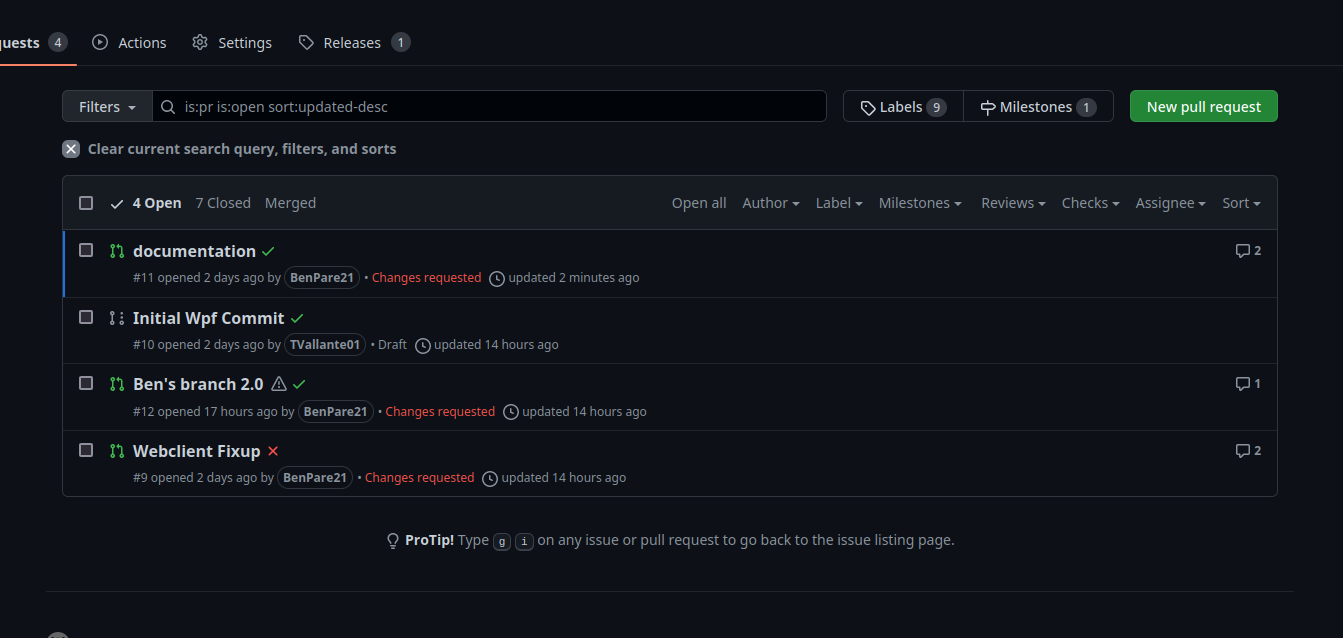
\includegraphics[width=9cm]{github.png}
        \end{column}
    \end{columns}

    \note{
        \huge{Joe}\normalsize

        We use github to manage our development process, as well as build docker images
        for the server, and binary images for use on client computers.
    }
\end{frame}

\begin{frame}
    \frametitle{Github (Pull Requests)}

    % Some columns
    \begin{columns}
        \begin{column}{0.58\textwidth}
            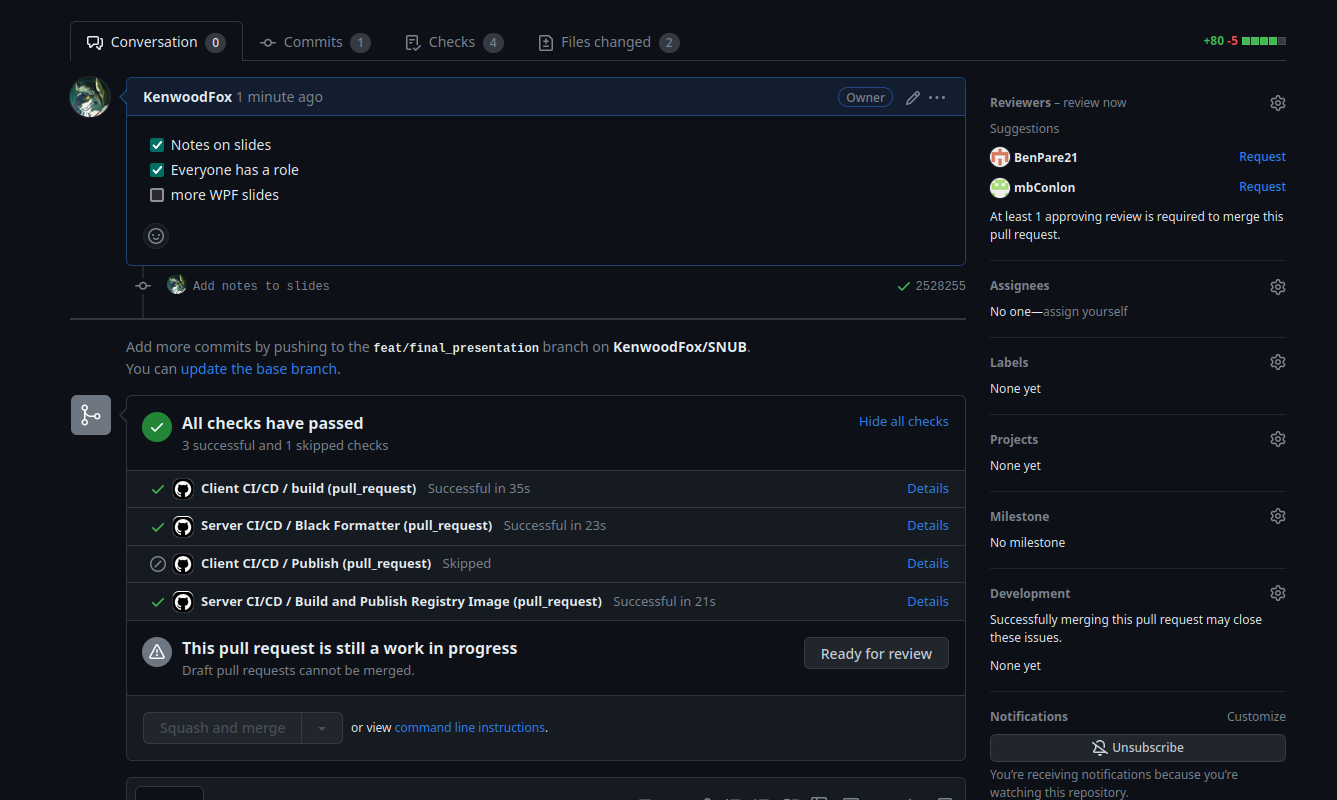
\includegraphics[width=9cm]{pullrequest.png}
        \end{column}
        \begin{column}{0.28\textwidth}
            \begin{block}{Pull Requests}
                Pull requests give every team member the chance to review changes
                to the code before they are implemented.
            \end{block}
        \end{column}
    \end{columns}

    \note{
        \huge{Joe}\normalsize

        Pull requests give every team member the chance to review changes
        to the code before they are implemented. This is especially important
        when using networked code, as one change may break compatability with
        the other portions of code!.
    }
\end{frame}

\begin{frame}
    \frametitle{Github (Commits)}

    % Some columns
    \begin{columns}
        \begin{column}{0.23\textwidth}
            \begin{block}{Commits}
                Each commit is a specific list of changes and differences (also called
                a patch) that can be shared around.
            \end{block}
        \end{column}
        \begin{column}{0.63\textwidth}
            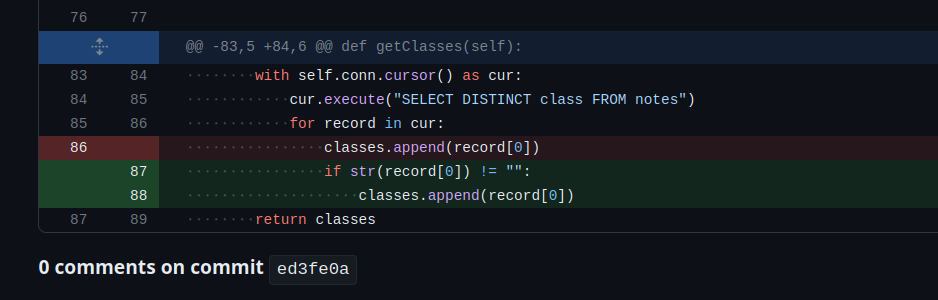
\includegraphics[width=10cm]{commit.png}
        \end{column}
    \end{columns}

    \note{
        \huge{Joe}\normalsize

        This patch here fixes a bug where empty strings may be returned when searching
        all classes.
    }
\end{frame}

\begin{frame}
    \frametitle{Alternative Clients}

    % Some columns
    \begin{columns}
        \begin{column}{0.38\textwidth}
            \begin{block}{WPF Client}
                Our unique server-side system allows for multiple different clients and a very even distribution of work.
            \end{block}
        \end{column}
        \begin{column}{0.58\textwidth}
            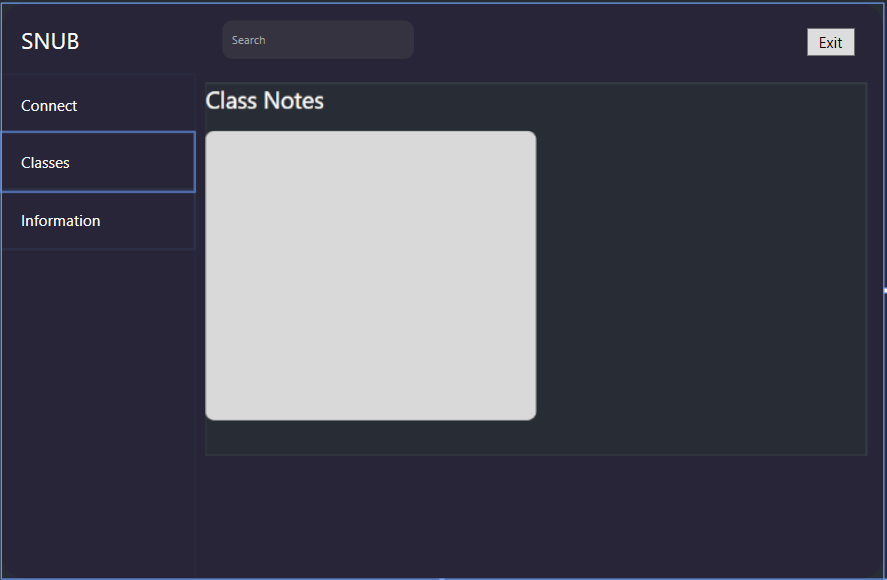
\includegraphics[width=9cm]{WpfBluePrint.png}
        \end{column}
    \end{columns}

    \note{
        \huge{Timm}\normalsize

        Talk about your client
    }
\end{frame}

\begin{frame}
    \frametitle{End}

    \begin{block}{}
        \begin{center}
            \Huge Questions and Comments?
        \end{center}
    \end{block}

    \begin{center}
        Find the source code for this document, and the rest of our designs, firmware, hardware
        and notes on GitHub!

        
\includegraphics[height=4cm]{github_qr}
    \end{center}

    \note{
        \huge{Everyone}\normalsize

        We will do demo afterward.

        Does anyone have questions?
    }
\end{frame}

\end{document}

